\section{Wechselrichter}
\subsection{Einphasig}
\textbf{Übung 7 Einphasiger Wechselrichter}\newline
\begin{tabular}{ p{.30\textwidth}  p{.2\textwidth} }       
        $\tau = \frac{L}{R} \qquad T = \frac{1}{f} \qquad \diff t = \frac{T}{N-1}$ \newline\newline&
        \\
            
        \textbf{Schaltzeitpunkte}&\\              
        $t_e(i) = (i-1) \cdot \diff t$\newline
        $t_a(i) = t_e(i) + k \cdot \diff t \cdot |\sin(\omega \cdot t_e(i))|$\newline\newline&
        \\
       
        \textbf{Laststrom} & \\          
        $i_L(t) = \frac{U_1}{R} \cdot \left( 1-e^{\frac{t_{ei}-t}{\tau}}\right) + i_L(t_{ei}) \cdot e^{\frac{t_{ei}-t}{\tau}}$&
        $t \in [t_{ei},t_{ai}]$
        \\
                  
        $i_L(t) = i_L(t_{ai}) \cdot e^{\frac{t_{ai}-t}{\tau}}$&
        $t \in [t_{ai},t_{ei+1}]$
        \\
\end{tabular}
\begin{minipage}{0.5\linewidth}
    \vspace{-2cm}
        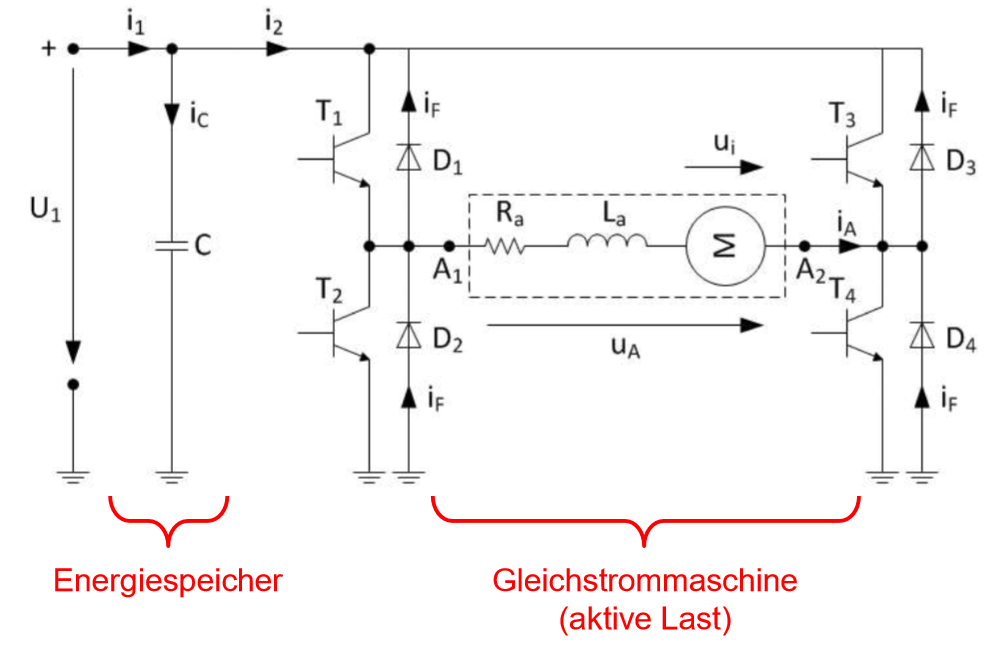
\includegraphics[width=0.9\linewidth]{images/WrEinphaseSchema}\newline
        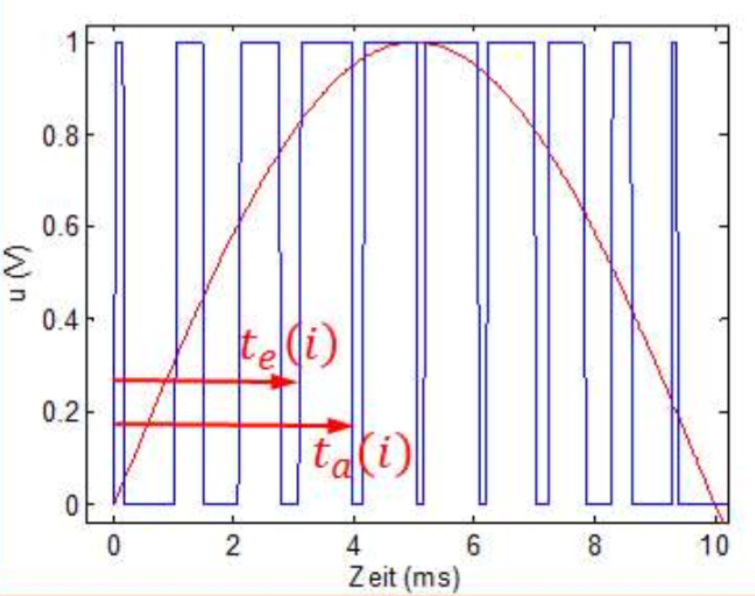
\includegraphics[width=0.5\linewidth]{images/WrEinphaseTime}
\end{minipage}
\clearpage